\chapter{Capitulo 1}
\justifying
\textbf{Introducción}: Consta de las siguientes secciones:
 	\begin{enumerate}
 		 \item Definiciones. 
 		 \item Ecuaciones de Conservación.
 		  \item Ecuacione Constitutiva. Ley de Fick.
 		   \item Balance de Masa. 
 		   \item Calculo de la Difusividad. 
 	   \end{enumerate} 
 	   \section{Definiciones} 
 	   \begin{itemize}
 	  \item \emph{$\rho_i$}: Concentración másica de la especie i (masa de i/volumen)
 	  \item $C_i$=$\frac{\rho_i}{\mu_i}$: Concentración molar de la especie i (moles/volumen)
 	  \item $w_i=\frac{\rho_i}{\rho}$: fracción masica de i ($\rho$ es la densidad de la solución)
 	  \item $x_i=\frac{C_i}{C}$: fracción molar ($C$ es la densidad molar total de la solución)
 	  \item \emph{$ \underline{v}_i$}: velocidad de la especie i con respecto a un sistema de coordenadas fijo. La velocidad promedio local \emph{$ \underline{v}$} se define como:
 	 \end{itemize}
 	 \begin{equation}
 	 \emph{$ \underline{v}=\frac{\sum_{i=1}^n \rho_i  \underline{v}_i}{\sum_{j=1}^n \rho_i}$}
 	 \tag{1.1}
     \label{eq_1.1}
 	  \end{equation}
 	  \emph{$\rho  \underline{v}$} = flux de masa. La velocidad promedio molar es:
 	   \begin{equation}
 	  	\emph{$ \underline{v}^*=\frac{\sum_{i=1}^n C_i  \underline{v_i}}{\sum_{i=1}^n C_i}$}
 	  	\tag{1.2}
        \label{eq_1.2}
 	  \end{equation}
 	
$C\underline{\emph{v}}=$flux molar de masa.
 \begin{equation}
 \underline{	{v}_i} -\underline{{v} }=\quad \text{velocidad de difusión de $i$ con respecto a ${v}$}. \tag{1.3}
 \label{eq_1.3}
 \end{equation}
 
 \begin{equation}
 	\underline{{v}_i} -\underline{{v}^*}=\quad \text{velocidad de difusión de $i$ con respecto a $\vec{v}^*$}. \tag{1.4} \label{eq_1.4}
 \end{equation}
 
 Con respecto a ejes estacionarios, los flujos de masa se definen de la siguiente manera:
 \begin{equation}
 	\underline{n}_i = \rho_i \underline{v}_i \quad \text{másico} \tag{1.5}
    \label{eq_1.5}
 \end{equation}
 \begin{equation}
 	\underline{N}_i = C_i \underline{v}_i \quad \text{molar} \tag{1.6}\label{eq_1.6}
 \end{equation}
 
 Con respecto a las velocidades promedio:
 \begin{equation}
 		\underline{{j}_i} = \rho_i (	\underline{{v}_i} -\underline{v}) \tag{1.7}\label{eq_1.7}
 \end{equation}
 \begin{equation}
 	\underline{{J}_i} = C_i (\underline{{v}_i} -	\underline{v}) \tag{1.8} \label{eq_1.8}
 \end{equation}
 
 Con respecto a las velocidades molares promedio:
 \begin{equation}
 	\underline{j}_i^* = \rho_i (\underline{v}_i - \underline{v}^*) \quad \text{másico} \tag{1.9} \label{eq_1.9}
 \end{equation}
 \begin{equation}
 	\underline{J}_i^* = C_i (\underline{v}_i - \underline{v}^*) \quad \text{molar} \tag{1.10} \label{eq_1.10}
 \end{equation}
 
 Relaciones entre los flujos molares. A partir de las ecs. \textbf{\eqref{eq_1.2}} y \textbf{\eqref{eq_1.10}} :
 \begin{equation}
 	\underline{J}_i^* = C_i (\underline{v}_i - \underline{v}^*) = C_i \underline{v}_i^* - \frac{C_i}{C} \sum_{j=1}^n C_j \underline{v}_j \tag{1.11} \label{eq_1.11}
 \end{equation}
 
 Por las relaciones (ecs. \textbf{\eqref{eq_1.6}} y $x_i$):
 \begin{equation}
 	\underline{J}_i^* = \underline{v}_i - x_i \sum_{j=1}^n x_j \underline{v}_j \tag{1.12}\label{eq_1.12}
 \end{equation}
 
 Para un sistema binario=$\underline{J}_A^*=\underline{N}_A-x_A (\underline{N_A}+\underline{N_B})$
 
 Para los fluxes másicos con respecto a \underline{\emph{v}} tenemos que: $\underline{J}_A=\underline{n}_A-w_A (\underline{n_A}+\underline{n_B})$

 A partir de la ec. \textbf{\eqref{eq_1.12}} se obtiene que:
 \begin{equation}
 	\sum_{i=1}^n \underline{J}_i^* =0 \tag{1.13}\label{eq_1.13}
 \end{equation}
 
 y para una mezcla binaria se obtiene:
 \begin{equation}
 	\underline{J}_A^* + \underline{J}_B^* = 0 \tag{1.14}\label{eq_1.14}
 \end{equation}
 
 Igualmente, la ec. \textbf{\eqref{eq_1.1}} puede ser escrita como:	
 
$\rho \underline{\emph{v}}=\rho_A \underline{\emph{v}}_A+\rho_B \underline{\emph{v}}_B=\underline{n}_B+\underline{n}_B$
 
 y la ec. \textbf{\eqref{eq_1.7}} puede ser expresada como:
 
 $ \underline{j}_A=	\rho_A \underline{v}_A + \rho_A \underline{v} \Rightarrow \underline{n}_A = \underline{j}_A + \rho_A \underline{v} $
 
 \section{Ecuaciones de Conservación}
 \textbf{Mezclas Binarias}
 
 La ecuación de continuidad para el componente $A$ en una mezcla binaria está dada por la siguiente ecuación:
 \begin{equation}
 	\frac{\partial \rho_A}{\partial t} + \nabla \cdot \underline{n}_A = r_A \tag{1.15}\label{eq_1.15}
 \end{equation}
 
 donde $\underline{n}_A=\rho_A \underline{v}_A$ es el flujo de masa.		 Similarmente, para el componente $B$:
 \begin{equation}
 	\frac{\partial \rho_B}{\partial t} + \nabla \cdot \underline{n}_B = r_B \tag{1.16}\label{eq_1.16}
 \end{equation}
 
 La adición de \textbf{\eqref{eq_1.15}} y \textbf{\eqref{eq_1.16}} (en donde  $\underline{n}_A + \underline{n}_B = \rho \underline{v}$ y $r_A + r_B = 0$)
 \begin{equation}
 	\frac{\partial \rho}{\partial t} + \nabla \cdot \rho \underline{v} = 0 \tag{1.17} \label{eq_1.17}
 \end{equation}
 
 que es la ecuación de continuidad o conservación de masa de la mezcla. En caso en que $\rho$ es constante:
 \begin{equation}
 	\nabla \cdot \underline{v} = 0 \tag{1.18}\label{eq_1.18}
 \end{equation}
 
 En términos de las variables molares:
 \begin{equation}
 	\frac{\partial C_A}{\partial t} + (\nabla \cdot \underline{N_A}) = R_A \tag{1.19} \label{eq_1.19}
 \end{equation}
 \begin{equation}
 	\frac{\partial C_B}{\partial t} + \nabla \cdot \underline{N}_B = R_B \tag{1.20} \label{eq_1.20}
 \end{equation}
 
 Adicionando:
 \begin{equation}
 	\frac{\partial C}{\partial t} + \nabla \cdot C {v}^* = R_A + R_B \tag{1.21} \label{eq_1.21}
 \end{equation}
 
 La ecuación \textbf{\eqref{eq_1.21}} supone que $\underline{N}_A +\underline{ N}_B = C \underline{v}^*$ y $R_A + R_B \neq 0$ si los moles no se conservan. Para un fluido de $C$ constante:
 \begin{equation}
 	\nabla \cdot \underline{v}^* = \frac{1}{C} (R_A + R_B) \tag{1.22}
    \label{eq_1.22}
 \end{equation}
 
 En el \underline{Apéndice A}, la ecuación \textbf{\eqref{eq_1.19}} se expresa en los tres sistemas de coordenadas.



 \section{Ecuación constitutiva: Ley de Fick}

Definiendo la difusividad másica $\mathscr{D}_{AB}=\mathscr{D}_{BA}$ en un sistema binario, la expresión del flux de masa es:
\begin{equation}
	\underline{J}_A^* = - \emph{C} \mathscr{D}_{AB} \nabla x_A  \tag{1.23}
    \label{eq_1.23}
\end{equation}
Análogamente,
\begin{equation}
	\underline{j}_A = - \rho \mathscr{D}_{AB} \nabla w_A  \tag{1.24}\label{eq_1.24}
\end{equation}

Esta es la primera ley de Fick de difusión. En términos de $N_A$ relativo a coordenadas estacionarias,
\begin{equation}
	\underline{N}_A = x_A (\underline{N}_A + \underline{N}_B) - \emph{C} \mathscr{D}_{AB} \nabla x_A  \tag{1.25}\label{eq_1.25}
\end{equation}


\begin{equation}
	\underline{n}_A = w_A (\underline{n}_A + \underline{n}_B) - \rho \mathscr{D}_{AB} \nabla w_A  \tag{1.26}\label{eq_1.26}
\end{equation}

 \section{Balance de Masa}
 Sustituyendo la ecuación \textbf{\eqref{eq_1.26}} en la ecuación \textbf{\eqref{eq_1.15}} se obtiene:
 \begin{equation}
 	\frac{\partial \rho_A}{\partial t} + \nabla \cdot \rho_A \underline{v} = \nabla \cdot \rho \mathscr{D}_{AB} \nabla w_A + r_A \tag{1.27}\label{eq_1.27}
 \end{equation}
 
 Similarmente, sustituyendo la ecuación \textbf{\eqref{eq_1.25}} en la ecuación \textbf{\eqref{eq_1.19}} se obtiene:
 \begin{equation}
 	\frac{\partial {C}_A}{\partial t} + \nabla \cdot C_A \underline{v}^* = \nabla \cdot C \mathscr{D}_{AB} \nabla x_A + R_A  \tag{1.28}\label{eq_1.28}
 \end{equation}
 
 Si $\rho$ y $\mathscr{D}_{AB}$ son constantes, entonces:
 \begin{equation}
 	\frac{\partial \rho_A}{\partial t} + \rho  (\nabla\cdot \underline{v})+\underline{v} \cdot \nabla \rho_A = \mathscr{D}_{AB} \nabla^2 \rho_A + r_A  \tag{1.29}\label{eq_1.29}
 \end{equation}
 
 donde $\nabla \cdot v = 0$ (Ec. \textbf{\eqref{eq_1.18}}). Dividiendo \textbf{\eqref{eq_1.29}} entre $M$ se obtiene:
 \begin{equation}
 	\frac{\partial C_A}{\partial t} + \underline{v} \cdot \nabla C_A = \mathscr{D}_{AB} \nabla^2 C_A + R_A  \tag{1.30} \label{eq_1.30}
 \end{equation}
 
 Esta ecuación se emplea comúnmente en soluciones diluidas líquidas. Si $C$ y $\mathscr{D}_{AB}$ son constantes, la ecuación \textbf{\eqref{eq_1.28}} se convierte en:
 \begin{equation}
 	\frac{\partial C_A}{\partial t} +C_A (\nabla \cdot \underline{v}^*)+ \underline{v}^*\cdot\nabla C_A  = \mathscr{D}_{AB} \nabla^2 C_A + R_A \tag {1.31}\label{eq_1.31}
 \end{equation}
 
 Como: $	\nabla \cdot \underline{v^*}= \frac{1}{c} (R_A + R_B) \quad \text{(Ver ec. \textbf{\eqref{eq_1.21})}}$
 
 Entonces:
 \begin{equation}
 	\frac{\partial C_A}{\partial t} + \underline{v}^* \cdot\nabla C_A=\mathscr{D}_{AB} \nabla^2 C_A+R_A-\frac{C_A}{C}(R_A+R_B) \tag{1.32}\label{eq_1.32}
 \end{equation}
 Si la velocidad es cero y no hay reacción química, se obtiene:
  \begin{equation}
 	\frac{\partial C_A}{\partial t}=\mathscr{D}_{AB} \nabla^2 C_A \tag{1.33}\label{eq_1.33}
 	\end{equation}
 	
 \section{Cálculo de la difusividad}
 \subsection{Teoría de la difusión de gases a baja densidad.}
 		Considerar un gas con moléculas A y A$^*$	que tienen la misma masa $m_A$
 		y el mismo tamaño y forma. Se plantea determinar la difusividad másica $\mathscr{D}_{AA^*}$
 		de un sistema de moléculas rígidas de diámetro $d_A$. Utilizando las definiciones obtenidas en el libro y en la teoría cinética de gases:
 	
 	Velocidad promedio:
 		\begin{equation}
 			\langle v \rangle = \sqrt{\frac{8k_B	T}{\pi m}}  \tag{1.34}\label{eq_1.34}
 		\end{equation}
 		$k_B=$Constante de Boltzman
 	
 	Frecuencia de colisiones:
 		\begin{equation}
 			Z = \frac{1}{4} n \langle v \rangle  \tag{1.35}\label{eq_1.35}
 		\end{equation}
 		Trayectoria libre media
 		\begin{equation}
 			\lambda = \frac{1}{\sqrt{2} \pi d^2 n}  \tag{1.36}\label{eq_1.36}
 		\end{equation}
 		Dado un dominio que contiene planos con encuadraciones diferentes separados por una distancia a, la relación entre a y $\lambda$ es:
 		 		\begin{equation}
 		 			a=\frac{2}{3} \lambda \tag{1.37}\label{eq_1.37}
 		 			\end{equation}
        \begin{figure}[h]

        \centering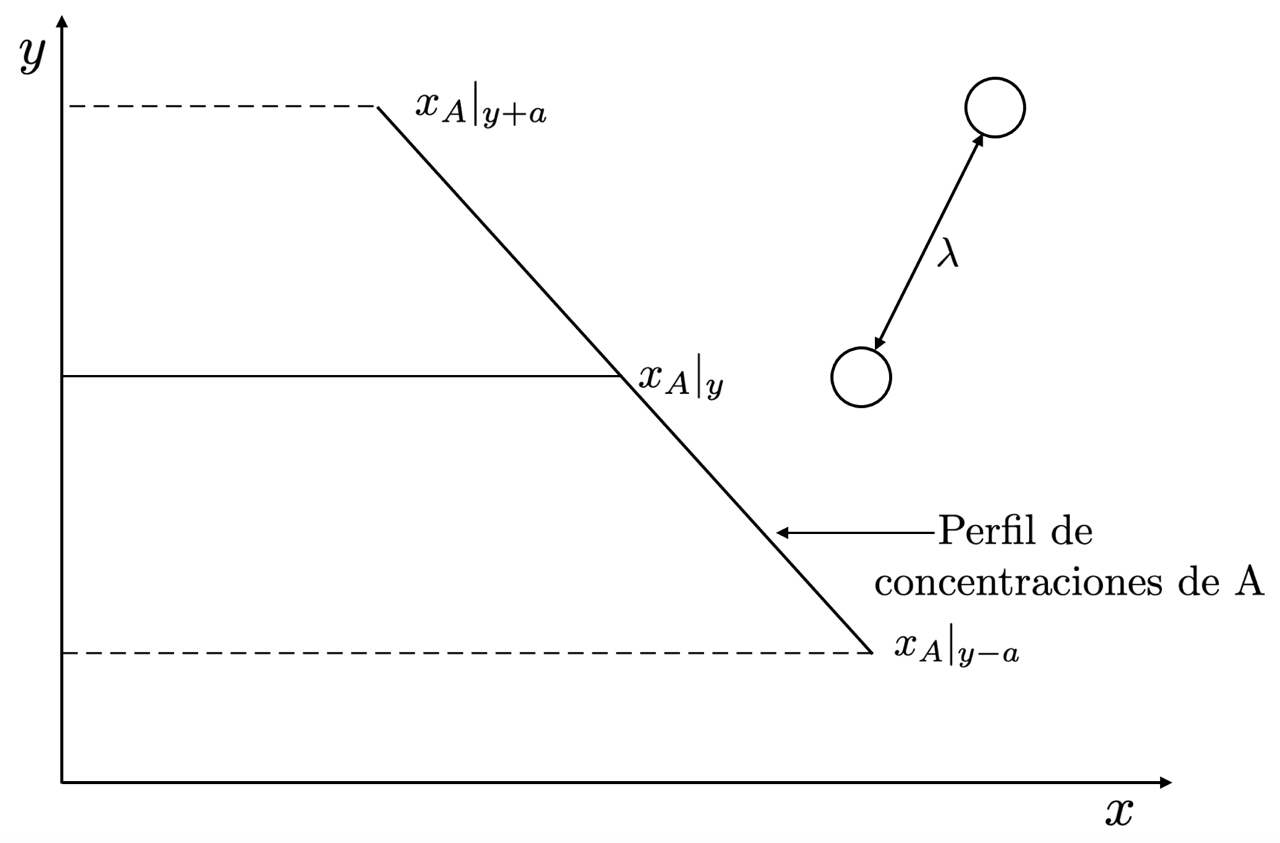
\includegraphics[width=0.6\linewidth]{Capitulo1/Imagenes/Fig_1.1.jpeg}
        \caption{Transferencia molecular de A del plano (y-a) al plano(y)}
        \label{fig:Fig_1.1}

\end{figure}

        
        El flux de masa de A efectivo entre el plano (y+a) y el plano (y-a) es:
        \begin{equation}
N_{A_{y}} = \frac{1}{\vec{N}} \left[ n x_A  v_y^* \bigg|_{y} + \frac{1}{4}n x_A \langle v \rangle \bigg|_{y-a}- \frac{1}{4} nx_A\langle v \rangle \bigg|_{y+a} \right]
\tag{1.38} \label{eq_1.38}
\end{equation}

Si el perfil de concentraciones es lineal, entonces:

\begin{equation}
x_A \bigg|_{y-a} = x_A \bigg|_{y-a} - \frac{2}{3}\lambda \frac{dx_A}{dy}
\tag{1.39} \label{eq_1.39}
\end{equation}

\begin{equation}
x_A \bigg|_{y+a} = x_A \bigg|_{y+a} + \frac{2}{3}\lambda \frac{dx_A}{dy}
\tag{1.40} \label{eq_1.40}
\end{equation}

Ya que \( Cv^* = N_A + N_B \), las ecs. \textbf{\eqref{eq_1.37}}, \textbf{\eqref{eq_1.38}}, \textbf{\eqref{eq_1.39}} y \textbf{\eqref{eq_1.40}} se combinan para dar:

\begin{equation}
N_{A_{y}} = x_A \left( N_{A_y} + N_{A_y}^* \right) - \frac{2}{3}C \langle v \rangle \lambda \frac{dx_A}{dy} \tag{1.41}\label{eq_1.41}
\end{equation}

De acuerdo con la ley de Fick:

\begin{equation}
\mathscr{D}_{AB} = \frac{1}{3} \langle v \rangle \lambda  \tag{1.42}\label{eq_1.42}
\end{equation}

Utilizando la ley de los gases ideales ( $P = CRT = nk_BT $) y las expresiones para \( \langle v \rangle \) y \( \lambda \), se obtiene para la autodifusión:

\begin{equation}
\mathscr{D}_{AA}^* = \frac{2}{3} \left( \frac{k_B^3}{\pi^3 m_A} \right)^{1/2} \frac{T^{3/2}}{P d_A^2}\tag{1.43}\label{eq_1.43}
\end{equation}

La ecuación \textbf{\eqref{eq_1.42}} representa la difusividad másica de una mezcla de dos especies de esferas rígidas de igual masa y diámetro. En el caso de diferentes masas y diámetros, la ecuación \textbf{\eqref{eq_1.43}} se generaliza:

\begin{equation}
\mathscr{D}_{AB} = \frac{2}{3} \left( \frac{k_B^3}{\pi^3} \right) \left( \frac{1}{2 m_A} + \frac{1}{2 m_B} \right)^{1/2} \frac{T^{3/2}}{P \left( \frac{d_A + d_B}{2} \right)^2}\tag{1.44}\label{eq_1.44}
\end{equation}

La teoría de Chapman-Enskog proporciona expresiones más exactas del coeficiente de difusión:

\begin{equation}
c \mathscr{D}_{AB} = (2.625 \times 10^{-5}) \frac{\sqrt{T(\frac{1}{M_A}+\frac{1}{M_B})}}{\sigma_{AB}^2 \Omega_{\mathscr{D}_{AB}}}\tag{1.45}\label{eq_1.45}
\end{equation}
Si C está dada por la ley de los gases ideales, entonces:

\begin{equation}
\mathscr{D}_{AB} = 0.00186 \sqrt{T^3(\frac{1}{M_A}+\frac{1}{M_B})}\frac{1}{P \sigma_{AB}^2 \Omega_{\mathscr{D}_{AB}}}  \tag{1.46}\label{eq_1.46}
\end{equation}

\(\Omega_{\mathscr{D}_{AB}}\) es una función adimensional de la temperatura y del potencial intermolecular entre moléculas \( A \) y \( B \). Este potencial se aproxima por el de Lennard-Jones:

\begin{equation}
\varphi_{AB}=4 \epsilon_{AB}[(\frac{\sigma_{AB}}{r})^{12}-(\frac{\sigma_{AB}}{r})^6]  \tag{1.47}\label{eq_1.47}
\end{equation}

En el Apéndice C se pueden encontrar tablas de \( \Omega_{\mathscr{D}_{AB}} \) en función de \( k_B / \epsilon_{AB} \). Para esferas rígidas, \( \Omega_{\mathscr{D}_{AB}} = 1 \). En mezclas binarias:

\begin{equation}
\sigma_{AB} = \frac{1}{2} (\sigma_A+\sigma_B)\tag{1.48}\label{eq_1.48}
\end{equation}

\begin{equation}
\epsilon_{AB} = \sqrt{\epsilon_A \epsilon_B}\tag{1.49}\label{eq_1.49}
\end{equation}

Las constantes $\sigma_{AB}$ y \( \epsilon_{AB} \) pueden ser identificadas en el Apéndice. En el caso de pares isotópicos:$\sigma_{AA^*}=\sigma_A=\sigma_A^*$  y  $\epsilon_{AA^*}=\epsilon_A=\epsilon_A^*$.




Si \( M_A = M_B \), la ecuación \eqref{eq_1.45} se reduce a:

\begin{equation}
C\mathscr{D}_{AA^*} = 3.2 \times 10^{-5}\sqrt{\frac{T}{M_A}} \frac{1}{\sigma_A \Omega_{\mathscr{D}_{AA^*}}} \tag{1.50}\label{eq_1.50}
\end{equation}

Definiendo el número de Schmidt:

\begin{equation}
Sc = \frac{\mu / \rho}{\mathscr{D}_{AB}} = \frac{\nu}{\mathscr{D_{AB}}} (\text{0.2 - 5 en gases}) \tag{1.51}\label{eq_1.51}
\end{equation}

Tenemos que:

\begin{equation}
\frac{\nu}{\mathscr{D}_{AA^*}} = \frac{5}{6}\frac{\Omega_{\mathscr{D}_{AA^*}}}{ \Omega_\mu}\tag{1.52}\label{eq_1.52}
\end{equation}

Por lo que: $\mathscr{D}_{AA^*} \approx 1.32 \nu$
\subsection{Dependencia de la difusividad de la presión y temperatura (PyT)}
En sistemas de mezclas de gases a bajas presiones,  $\mathscr{D}_{AB}$ es inversamente proporcional a P, directamente proporcional a T e independiente de la concentración de un par de gases.
Utilizando estados correspondientes y la teoría cinética, \( \mathscr{D}_{AB} \) está dado por la siguiente ecuación:
\setcounter{figure}{50}
\begin{equation}
\frac{P \mathscr{D}_{AB}}{(P_{C_A} P_{C_{B}})^{1/5} (T_{{C_B}} T_{C_{B}})^{5/12} \left( \frac{1}{M_A} + \frac{1}{M_B} \right)^{1/2}} = a \left( \frac{T}{T_{C_A} T_{C_B}} \right)^b\tag{1.53}\label{eq_1.53}
\end{equation}

Gases no polares: \( a = 2.745 \times 10^{-4} \) y \( b = 1.823 \)  

H$_2$O + gas no polar: \( a = 3.64 \times 10^{-4} \) y \( b = 2.334 \)

En la figura \textbf{\eqref{fig:Fig_1.51}} se grafica \( C \mathscr{D}_{AA^*}\) como función de \( T_R \) y \( P_R \) (T y P reducidas), \( (C \mathscr{D}_{AA^*})_R=\frac{C\mathscr{D}_{AA^*}}{(C\mathscr{D}_{AA^*)_c}} \) .
$((\mathscr{D})_c \text{es la cantidad crítica})$

$(C\mathscr{D}_{AA^*})_c$ coeficiente de difusión crítico puede ser estimado por la siguiente ecuación:

\begin{equation}
(C\mathscr{D}_{AA^*})_c = 2.96 \times 10^{-6} \left( \frac{1}{M_A} + \frac{1}{M_{A^*}} \right)^{1/2} \frac{P_{cA}^{1/3}}{T_{cA}^{1/6}}\tag{1.54}\label{eq_1.54}
\end{equation}

En el caso de gases \( A \) y \( B \), la ecuación \textbf{\eqref{eq_1.54}} puede reducirse a la aproximación siguiente:

\begin{equation}
(C \mathscr{D}_{AA^*}) = 2.96 \times 10^{-6} \left( \frac{1}{M_A} + \frac{1}{M_B} \right)^{1/2}  \frac{(P_{cA} P_{cB})^{1/3}}{(T_{cA} T_{cB})^{1/12}} \tag{1.55}\label{eq_1.55}
\end{equation}

Correspondientemente, en el caso de A y B en la figura \textbf{\eqref{fig:Fig_1.51}}
$T_R=\frac{T}{\sqrt{T_{cA}T_{cB}}}$ y $P_R=\frac{P}{\sqrt{P_{cA}P_{cB}}}$
\begin{figure}[H]
\centering
        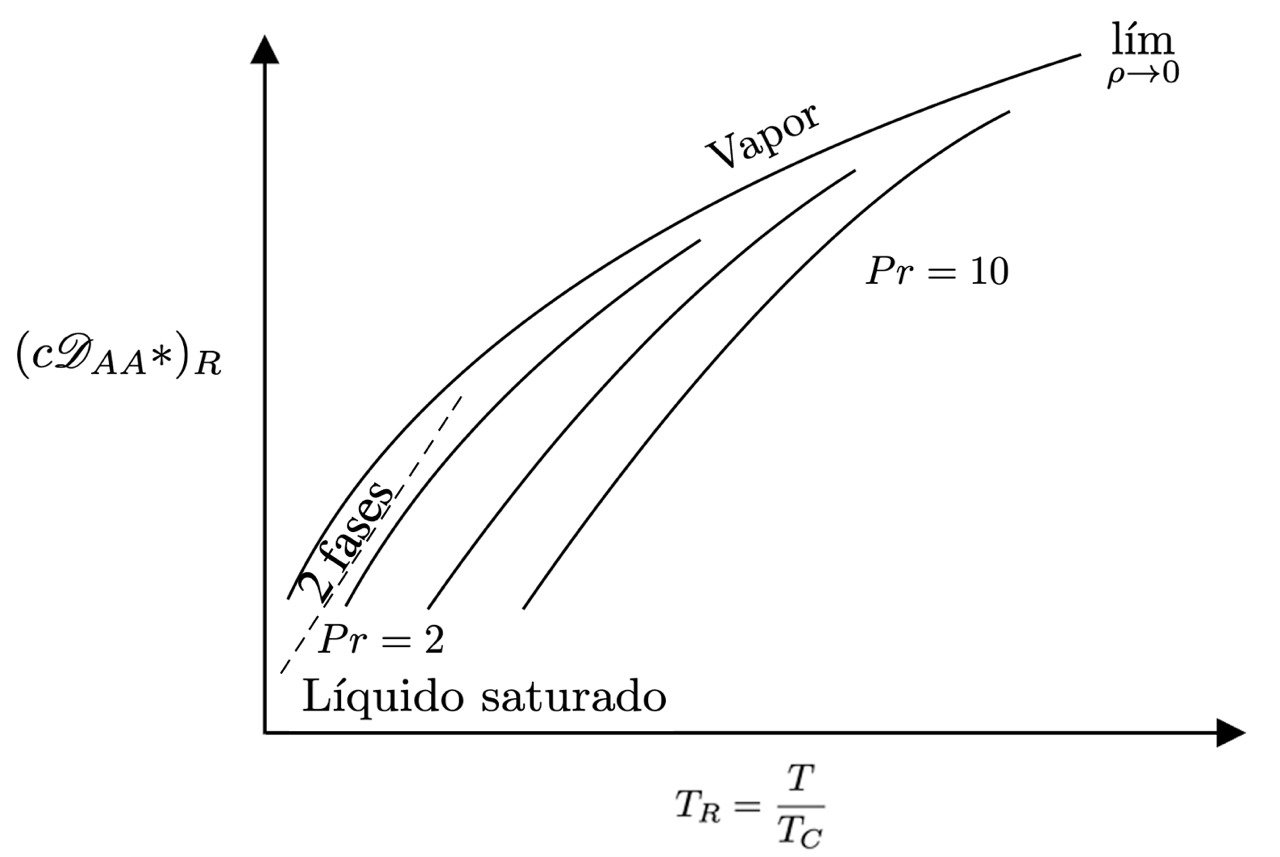
\includegraphics[width=0.7
        \linewidth]{Capitulo1/Imagenes/Fig_1.51.jpeg}
        \caption{Mezclador estático (a) y mezclador dinámico (b)}
        \label{fig:Fig_1.51}

\end{figure}

\subsubsection{Teoría de la difusión en líquidos binarios}
La teoría hidrodinámica se basa en la ecuación de Nernst-Einstein, que postula que la difusividad de una partícula A (el soluto) en un medio estacionario B está expresado como:

\begin{equation}
\mathscr{D}_{AB} = k_B T \frac{U_A}{F_A}\tag{1.56}\label{eq_1.56}
\end{equation}

en donde $U_A/F_A $ es la movilidad de la partícula A. Si A es esférica y además existe deslizamiento en la interfase sólido-fluido, se obtiene:

\begin{equation}
\frac{U_A}{F_A} = \frac{(3 \mu_B + R_A \beta_{AB})}{({2 \mu_B + R_A \beta_{AB}} )}  \frac{1}{6 \pi \mu_B R_A}\tag{1.57}\label{eq_1.57}
\end{equation}

en donde \( \mu_B \) es la viscosidad del solvente, \( R_A \) es el radio de la partícula y \( \beta_{AB} \) es el coeficiente de fricción interfacial. Hay 2 casos:

a)-.$( \beta_{AB} = \infty )$ (sin deslizamiento).
   En este caso, la ecuación \textbf{\eqref{eq_1.56}} se reduce a la ecuación de Stokes-Einstein:

   \begin{equation}
   \mathscr{D}_{AB} = \frac{k_B T}{6 \pi \mu_B R_A}\tag{1.58}\label{eq_1.58}
   \end{equation}

b)-. \( \beta_{AB} = 0 \) (con deslizamiento).  

   En este caso, la ecuación \textbf{\eqref{eq_1.56}} se reduce a:

   \begin{equation}
   \mathscr{D}_{AB} = \frac{k_B T}{4 \pi \mu_B R_A}\tag{1.59}\label{eq_1.59}
   \end{equation}

Si A y B son iguales, en un arreglo cúbico se obtiene:


$2 R_A = \left( \frac{\widetilde{V}_A}{\widetilde{N}_A} \right)^{1/3}$ y luego:

\begin{equation}
\mathscr{D}_{AB} = \frac{k_B T}{2 \pi \mu_A} \left( \frac{\widetilde{V}_A}{\widetilde{N}_A} \right)^{1/3}\tag{1.60}\label{eq_1.60}
\end{equation}

La teoría de Eyring del "estado activado" postula un estado "cuasicristalino" del líquido. Esta teoría deduce el siguiente resultado dentro del contexto de mecánica estadística:

\begin{equation}
\frac{\mathscr{D}_{AB} \mu_B}{(\mathscr{D}_{AB}\mu_B)_{X_A \to 0}} = \left[ 1 + X_A \frac{\widetilde{V}_A}{\widetilde{V}_B} \right] \left( \frac{\partial \ln \gamma_{A}}{d X_A} \right)_{T,P}\tag{1.61}\label{eq_1.61}
\end{equation}
en donde $\widetilde{V}_A$ y $\widetilde{V}_B$ son los volúmenes parciales molares de A y B, $\gamma_A$ es el coeficiente de actividad de A y $\mathscr{D}_{AB}$,$\mu_A$ son la difusividad y viscocidad de la mezcla.

Expresiones empíricas sugeridas para situaciones reales han sido propuestas. Por ejemplo, la ec. de Wilke-Chang:
\begin{equation}
    \mathscr{D}_{AB}=7.4\times10^{-8}\frac{\sqrt{\psi_BM_B}}{\mu \widetilde{V}_A^{0.6}}T
\tag{1.62}\label{eq_1.62}
\end{equation}
donde $\psi_B$ es el "parametro de asociación" del solvente.

$\psi_B=2.6$ para agua y 1.9 para metanol.
$\psi_B=1$ para solventes no asociativos. $\widetilde{V}_A=M_A/\rho$ y $\mu$ esta dada en cp.
\section{Tarea 1}
Bird et all 17.A
\begin{itemize}
\item[1.-] Predicción binaria a baja densidad. 
    Estimar $D_{AB}$  para el sistema metano-etano a 293°K y 1 atm por medio de los siguientes métodos.
    \begin{itemize}
        \item [a)-] Ecuación 1.53
        \item [b)-] Ecuación 1.53 y gráfica Fig 1.51 utilizando las T y P reducidas $T_{r}=\frac{T}{\sqrt{T_{CA}T_{CB}}}$ , $P_{r}=\frac{P}{\sqrt{P_{CA}P_{CB}}}$
        \item [c)-] Ecuación 1.46, 1.48 y 1.49, y los parámetros de Lennard-Joues del Apéndice C.
        \item [d)-] Ecuación 1.46 en los parámetros de Lennard-Jones estimados a partir de las propiedades críticas siguientes:
         $$\frac{\epsilon}{k_{13}}=0.77\sqrt{T_{CA}T_{CB}}  ,  T=\frac{2.44}{2} \left[ \left(\frac{T_{CA}}{P_{CA}}\right)^{1/5}+\left(\frac{T_{CB}}{P_{CB}}\right)^{1/3} \right] $$
    \end{itemize} 
    Respuestas ($cm^2/s$) : a)- 0.152; b)- 0.138; c)- 0.146; d)- 0.138
\item[2.-] Autodifusión de mercurio líquido Bird et all 17 A3.
La difusividad del $Hg^{203}$ en mercurio líquido normal se ha medido con datos de viscosidad y volumen másico. Comparar los datos experimentales con aquellos obtenidos 
por la ec. 160.
    \begin{table}[H]  %Aquí empieza la tabla%
    \centering  %Le digo  que se centre %
    \begin{tabular}{cccc}
    \hline
    \textbf{T(K)} & \textbf{$ D_{AB} $ $cm^2/s$} & \textbf{$\mu$ cP} & \textbf{$\hat{V}$ $cm^3/s$} \\ \hline
            275.7 & $1.52 \times 10^{-5}$ & 1.68 & 0.0736 \\ 
            289.6 & $1.68 \times 10^{-5}$ & 1.56 & 0.0737 \\ 
            364.2 & $2.57 \times 10^{-5}$ & 1.27 & 0.0748 \\ \hline
        \end{tabular}
    \end{table}  

Bird et all 17.A.5    
\item[3.-] Cálculo de la difusividad de una muestra binaria a alta densidad. 
Predecir $pD_{AB}$ para una mezcla equimolar de $N_{2}$ y $C_{2}H_{6}$ a 288.2 K y 40 atm.
    \begin{itemize}
     \item [a)-] Usar el valor de $D_{AB}$ a 1 atm de  0.148 $cm^2/s$ a T=298.2 Ky la gráfica de la Fig.1.51
     \item [b)-] Usar la ecuación 1.55 y la Fig 1.51
    \end{itemize}    
Respuesta a).- $5.8*10^{-6}$ gmol/cms; b).- $5.3*10^{-6}$ gmol/cms
\item[4.-] Prob. 17.A.6 Bird
Difusividad y número de Schmidit para mezclas cloro-aire. 
    \begin{itemize}
    \item [a)-] Predecir $D_{AB}$ para mezclas cloro-aire a 75°F y 1 atm.
    Utilizar los parámetros del Apéndice C.
    \item [b)-] Calcular (a) utilizando la ec. 1.53
    \item [c)-]Utilizar los resultados de (a) para estimar los valores del número de Schmidit para mezclas cloro-aire a 297 K y 1 atm para las siguientes fracciones mol y viscosidades:
    0, $1.83*10^{-4} poises$; 0.25, $1.64*10^{-4} poises$; 0.5, $1.5*10^{-4} poises$; 0.75, $1.39x10^{-4} poises$; 1, $1.31*10^{-4} poises$
    $$ pD_{AB}= \frac{\rho}{RT}D_{AB}; \space  Sc=\frac{\mu}{M_{C}D_{AB}}=\frac{\mu}{(x_{A}M_{A}+x_{B}M_{B})pD_{AB}}$$
\end{itemize}
Respuestas: a).- 0.121 $cm/s$; b).- 0.124 $cm/s$; c).- Sc=1.27, 0.832, 0.602, 0.463, 0.372
\item[5.-] Probl. 17.A.8 Bird.
Corrección para la difusividad a altas densidades. 
El valor medido para $pD_{AB}$ de una mezcla de 80\% mol de $CH_{4}$ Y 20\% mol de $C_{2}H_{6}$ a 313 K y 136 atm es $6x10^-6$ gmol/cms.
Calcular $pD_{AB}$ para esa mezcla a 136 atm y 351 K usando la Fig 1.51.

Respuesta $6.3*10^{-6} gmol/cm s$. Observado $6.33*10^{-6 }gmol/cm s$
\item[6.-]   Probl 17 A.10 Bird 
Cálculo de difusividad de líquidos 
\begin{itemize}
     \item [a)-] Calcular la difusividad de una solución diluida de ácido acético a 12.5°C utilizando la ec. 1.62. La densidad del ácido acético es 0.937 $g/cm^3$ en el punto de ebullición.
     \item [b)-] La difusividad de una solución diluida de metanol a 15°C es $1.28*10^{-5} cm^2/s$. Calcular la difusividad de esa solución a 100°C. 
     Las viscosidades a 15°C y 100°C son 1.14 cp y 0.28cp.
     La viscosidad de la solución diluida es 1.22 cp.
    \end{itemize}
Respuesta (b).- $6.7*10^{-5} cm^2/s$.
\end{itemize}
\newpage


 
\section{Apéndice A}
Ecuaciones de continuidad en varios sistemas de coordenadas

\subsection*{Coordenadas rectangulares:}
\begin{equation} \frac{\partial c_A}{\partial t} + \left( \frac{\partial N_{Az}}{\partial x} + \frac{\partial N_{Ay}}{\partial y} + \frac{\partial N_{Az}}{\partial z} \right) = R_A \tag{A}
\end{equation}

\subsection*{Coordenadas cilíndricas:}
\begin{equation} \frac{\partial c_A}{\partial t} + \left( \frac{1}{r} \frac{\partial}{\partial r} (rN_{Ar}) + \frac{1}{r} \frac{\partial N_{A\theta}}{\partial \theta} + \frac{\partial N_{Az}}{\partial z} \right) = R_A \tag{B} 
\end{equation}

\subsection*{Coordenadas esféricas:}
\begin{equation} \frac{\partial c_A}{\partial t} + \left( \frac{1}{r^2} \frac{\partial}{\partial r} (r^2 N_{Ar}) + \frac{1}{r \sin \theta} \frac{\partial}{\partial \theta} (N_{A\theta} \sin \theta) + \frac{1}{r \sin \theta} \frac{\partial N_{A\phi}}{\partial \phi} \right) = R_A \tag{C}
\end{equation}

\newpage
\section{Apéndice B}
Ecuación de continuidad de A con $\rho$ y $\mathcal{D}_{AB}$ constantes
\subsection*{Coordenadas rectangulares:}
\begin{equation}  \frac{\partial c_A}{\partial t} + \left( v_x \frac{\partial c_A}{\partial x} + v_y \frac{\partial c_A}{\partial y} + v_z \frac{\partial c_A}{\partial z} \right) = \mathcal{D}_{AB} \left( \frac{\partial^2 c_A}{\partial x^2} + \frac{\partial^2 c_A}{\partial y^2} + \frac{\partial^2 c_A}{\partial z^2} \right) + R_A \tag{A}
\end{equation}

\subsection*{Coordenadas cilíndricas:}
\begin{equation} 
    \begin{split} 
    \frac{\partial c_A}{\partial t} + &\left( v_r \frac{\partial c_A}{\partial r} + v_0 \frac{1}{r} \frac{\partial c_A}{\partial \theta} + v_z \frac{\partial c_A}{\partial z} \right) \\
      &= \mathcal{D}_{AB} \left( \frac{1}{r} \frac{\partial}{\partial r} \left( r \frac{\partial c_A}{\partial r} \right) + \frac{1}{r^2} \frac{\partial^2 c_A}{\partial \theta^2} + \frac{\partial^2 c_A}{\partial z^2} \right) + R_A
    \end{split} 
    \tag{B}
\end{equation}

\subsection*{Coordenadas esféricas:}
\begin{equation}
    \begin{split}
        \frac{\partial c_A}{\partial t} &+ \left( v_r \frac{\partial c_A}{\partial r} + v_{\theta} \frac{1}{r} \frac{\partial c_A}{\partial \theta} + v_\phi \frac{1}{r \sin \theta} \frac{\partial c_A}{\partial \phi} \right) \\
        &= \mathcal{D}_{AB} \left( \frac{1}{r^2} \frac{\partial}{\partial r} \left( r^2 \frac{\partial c_A}{\partial r} \right) + \frac{1}{r^2 \sin \theta} \frac{\partial}{\partial \theta} \left( \sin \theta \frac{\partial c_A}{\partial \theta} \right) + \frac{1}{r^2 \sin^2 \theta} \frac{\partial^2 c_A}{\partial \phi^2} \right) + R_A 
    \end{split}
    \tag{C}
\end{equation}

\begin{landscape} % Inicia la página en orientación horizontal
\section{Apéndice C} 
Tablas de Lennard-Jones y gases de baja densidad
\pagestyle{empty} % Elimina el encabezado en esta página

%\begin{longtable}{lccccccccc}
\begin{longtable}{p{2.6cm}p{1.3cm}|p{1.5cm}p{1.5cm}p{0.5cm}|p{1.5cm}p{1.5cm}p{1.5cm}|p{2cm}p{1.8cm}}
\caption{Parámetros Potenciales de Lennard-Jones  y Propiedades Críticas} \\
\toprule
 & \multicolumn{5}{c}{Parámetros Lennard-Jones} & \multicolumn{4}{c}{Propiedades Críticas$^{g,h}$} \\
\cmidrule(lr){2-5} \cmidrule(lr){6-10}
Susustancia &Masa Molar $M$& $\sigma$ (\AA) & $\epsilon/K$ (K) & Ref. & $T_c$ (K) & $p_c$ (atm) & $\tilde{V}_c$ (cm$^3$/g-mole) & $\mu_c$ \space (g/cm$\cdot$s$\times10^6$) & $k_c$ (cal/cm$\cdot$s$\cdot$K$\times 10^5$) \\
\midrule
\endfirsthead % Encabezado en la primera página
\multicolumn{10}{c}{{\bfseries \tablename\ \thetable{} -- Continuación}} \\
\toprule
 & \multicolumn{5}{c}{Parámetros Lennard-Jones } & \multicolumn{4}{c}{Propiedades Críticas$^{g,h}$} \\
\cmidrule(lr){2-5} \cmidrule(lr){6-10}
Susustancia &Masa Molar $M$& $\sigma$ (\AA) & $\epsilon/K$ (K) & Ref. & $T_c$ (K) & $p_c$ (atm) & $\tilde{V}_c$ (cm$^3$/g-mole) & $\mu_c$ \space (g/cm$\cdot$s$\times10^6$) & $k_c$ (cal/cm$\cdot$s$\cdot$K$\times 10^5$) \\
\midrule
\endhead % Encabezado en las páginas siguientes
\midrule
\multicolumn{10}{r}{{Continúa en la siguiente página}} \\
\endfoot % Pie de página en todas las páginas excepto la última
\bottomrule
\endlastfoot 

% Contenido de la tabla
\multicolumn{10}{l}{\textbf{Elementos ligeros:}} \\
H$_2$ & 2.016 & 2.915 & 38.0 & a & 33.3 & 12.80 & 65.0 & 34.7 & — \\
He & 4.003 & 2.576 & 10.2 & a & 5.26 & 2.26 & 57.8 & 25.4 & — \\
\midrule
\multicolumn{10}{l}{\textbf{Gases nobles:}} \\
Ne & 20.180 & 2.789 & 35.7 & a & 44.5 & 26.9 & 41.7 & 156. & 79.2 \\
Ar & 39.948 & 3.432 & 122.4 & b & 150.7 & 48.0 & 75.2 & 264. & 71.0 \\
Kr & 83.80 & 3.675 & 170.0 & b & 209.4 & 54.3 & 92.2 & 396. & 49.4 \\
Xe & 131.29 & 4.009 & 234.7 & b & 289.8 & 58.0 & 118.8 & 490. & 40.2 \\
\midrule
\multicolumn{10}{l}{\textbf{Gases poliatómicos simples:}} \\
Aire & 28.964 & 3.617 & 97.0 & a & 132.4 & 37.0 & 86.7 & 193. & 90.8 \\
N$_2$ & 28.013 & 3.667 & 99.8 & b & 126.2 & 33.5 & 90.1 & 180. & 86.8 \\
O$_2$ & 31.999 & 3.433 & 113. & a & 154.4 & 49.7 & 74.4 & 250. & 106.3 \\
CO & 28.010 & 3.590 & 110. & a & 132.9 & 34.5 & 93.1 & 190. & 86.5 \\
CO$_2$ & 44.010 & 3.996 & 190. & a & 304.2 & 72.8 & 94.1 & 343. & 122. \\
NO & 30.006 & 3.470 & 119. & a & 180. & 64. & 57. & 258. & 118.2 \\
N$_2$O & 44.012 & 3.879 & 220. & a & 309.7 & 71.7 & 96.3 & 332. & 131. \\
SO$_2$ & 64.065 & 4.026 & 363. & c & 430.7 & 77.8 & 122. & 411. & 98.6 \\
F$_2$ & 37.997 & 3.653 & 112. & a & — & — & — & — & — \\
Cl$_2$ & 70.905 & 4.115 & 357. & a & 417. & 76.1 & 124. & 420. & 97.0 \\
Br$_2$ & 159.808 & 4.268 & 520. & a & 584. & 102. & 144. & — & — \\
I$_2$ & 253.809 & 4.362 & 550. & a & 800. & — & — & — & — \\
\midrule
\multicolumn{10}{l}{\textbf{Hidrocarburos:}} \\
CH$_4$ & 16.04 & 3.780 & 154. & b & 191.1 & 45.8 & 98.7 & 159. & 158. \\
$\mathrm{CH} \equiv \mathrm{CH}$ & 26.04 & 4.114 & 212. & d & 308.7 & 61.6 & 112.9 & 237. & — \\
$\mathrm{CH_2}=\mathrm{CH_2}$ & 28.05 & 4.228 & 212. & b & 282.4 & 50.0 & 124. & 215. & — \\
C$_2$H$_6$ & 30.07 & 4.388 & 232. & b & 305.4 & 48.2 & 148. & 210. & 203. \\
$\text{CH}_3\text{C} \equiv \text{CH}$& 40.06 & 4.742 & 261 & d & 394.8 & — & — & — & — \\
$\text{CH}_3\text{CH} = \text{CH}_2$& 42.08 & 4.766 & 275. & b & 365.0 & 45.5 & 181. & 233. & — \\
n-C$_4$H$_{10}$ & 58.12 & 5.604 & 304. & b & 425.2 & 37.5 & 295. & 239. & — \\
i-C$_4$H$_{10}$ & 58.12 & 5.393 & 295. & b & 408.1 & 36.0 & 263. & 239. & — \\
n-C$_5$H$_{12}$ & 72.15 & 5.850 & 326. & b & 469.5 & 33.2 & 311. & 238. & — \\
i-C$_5$H$_{12}$ & 72.15 & 5.812 & 327. & b & 460.4 & 33.7 & 306. & — & — \\
C(CH$_3$)$_4$ & 72.15 & 5.759 & 312. & b & 433.8 & 31.6 & 303. & — & — \\
n-C$_6$H$_{14}$ & 86.18 & 6.264 & 342. & b & 507.3 & 29.7 & 370. & 248. & — \\
n-C$_7$H$_{16}$ & 100.20 & 6.663 & 352. & b & 540.1 & 27.0 & 432. & 254. & — \\
n-C$_8$H$_{18}$ & 114.23 & 7.035 & 361. & b & 568.7 & 24.5 & 492. & 259. & — \\
n-C$_9$H$_{20}$ & 128.26 & 7.463 & 351. & b & 594.6 & 22.6 & 548. & 265. & — \\
Ciclohexano & 84.16 & 6.143 & 313. & d & 553. & 40.0 & 308. & 284. & — \\
Benceno & 78.11 & 5.443 & 387. & b & 562.6 & 48.6 & 260. & 312. & — \\
\midrule
\multicolumn{10}{l}{\textbf{Otros compuestos orgánicos:}} \\
CH$_4$ & 16.04 & 3.780 & 154. & b & 191.1 & 45.8 & 98.7 & 159. & 158. \\
CH$_3$Cl & 50.49 & 4.151 & 355. & c & 416.3 & 65.9 & 143. & 338. & — \\
CH$_2$Cl$_2$ & 84.93 & 4.748 & 398. & c & 510. & 60. & — & — & — \\
CHCl$_3$ & 119.38 & 5.389 & 340. & e & 536.6 & 54. & 240. & 410. & — \\
CCl$_4$ & 153.82 & 5.947 & 323. & e & 556.4 & 45.0 & 276. & 413. & — \\
C$_2$N$_2$ & 52.034 & 4.361 & 349. & e & 400. & 59. & — & — & — \\
COS & 60.076 & 4.130 & 336. & e & 378. & 61. & — & — & — \\
CS$_2$ & 76.143 & 4.483 & 467. & e & 552. & 78. & 170. & 404. & — \\
CCl$_2$F$_2$ & 120.91 & 5.116 & 280. & b & 384.7 & 39.6 & 218. & — & — \\
\bottomrule
\end{longtable}

\footnotetext[1]{a) J. O. Hirschfelder, C. F. Curtiss, and R. B. Bird, \emph{Molecular Theory of Gases and Liquids}, corrected printing with notes added, Wiley, New York (1964).}
\footnotetext[2]{b) L. S. Tee, S. Gotoh, and W. E. Stewart, \textit{Ind. Eng. Chem. Fundamentals}, \textbf{5}, 356--363 (1966). The values for benzene are from viscosity data on that substance. The values for other substances are computed from Correlation (iii) of the paper.}
\footnotetext[3]{c) L. Monchick and E. A. Mason, \textit{J. Chem. Phys.}, \textbf{35}, 1676--1697 (1961); parameters obtained from viscosity.}
\footnotetext[4]{d) L. W. Flynn and G. Thodos, \textit{AIChE Journal}, \textbf{8}, 362--365 (1962); parameters obtained from viscosity.}
\footnotetext[5]{e) R. A. Svehla, \textit{NASA Tech. Report R-132} (1962); parameters obtained from viscosity. This report provides extensive tables of Lennard-Jones parameters, heat capacities, and calculated transport properties.}
\footnotetext[6]{f) Values of the critical constants for the pure substances are selected from K. A. Kobe and R. E. Lynn, Jr., \textit{Chem. Rev.}, \textbf{52}, 117--236 (1962); \textit{Amer. Petroleum Inst. Research Proj.} \textbf{44}, Thermodynamics Research Center, Texas A\&M University, College Station, Texas (1966); and \textit{Thermodynamic Functions of Gases}, F. Din (editor), Vols. 1--3, Butterworths, London (1956, 1961, 1962).}
\footnotetext[7]{g) Values of the critical viscosity are from O. A. Hougen and K. M. Watson, \textit{Chemical Process Principles}, Vol. 3, Wiley, New York (1947), p. 873.}
\footnotetext[8]{h) Values of the critical thermal conductivity are from E. J. Owens and G. Thodos, \textit{AIChE Journal}, \textbf{3}, 454--461 (1957).}
\footnotetext[9]{i) For air, the molecular weight \(M\) and the pseudocritical properties have been computed from the average composition of dry air as given in COESA, \textit{U.S. Standard Atmosphere 1976}, U.S. Government Printing Office, Washington, D.C. (1976).}
 
\newpage
\end{landscape}
\pagestyle{plain} % Restaura el encabezado
\begin{longtable}{p{1cm}p{1.8cm}p{2cm}|p{1.3cm}p{1.8cm}p{2cm}}
    \caption{Integrales de Colisión para su uso con los potenciales de Lennard-Jones para la predicción de propiedades de transporte de Gases de baja Densidad. \textsuperscript{a,b,c}} \\
    \hline
     %& \multicolumn{2}{c|}{} & \multicolumn{2}{c|}{\(\Omega_{b}=\Omega_{t}\)} \\
    \cline{2-3} \cline{4-5}
    KT/\(e\) &  \(\Omega_{\mu}=\Omega_{k}\) (por viscosidad y conductividad térmica) & \(\Omega_{D_{AB}}\) (por difusividad) & kT/\(e\) o KT/\(\varepsilon_{AB}\) & \(\Omega_{b}=\Omega_{k}\) (por viscosidad y conductividad térmica) & \(\Omega_{D_{AB}}\) (por difusividad) \\
    \hline
    \endfirsthead
    
    \multicolumn{6}{c}%
    {{\bfseries \tablename\ \thetable{} -- Continuación}} \\
    \hline
     %& \multicolumn{2}{c|}{\(\Omega_{s}=\Omega_{t}\)} & \multicolumn{2}{c|}{\(\Omega_{b}=\Omega_{t}\)} \\
    \cline{2-3} \cline{4-5}
    KT/\(e\) &  \(\Omega_{\mu}=\Omega_{k}\) (por viscosidad y conductividad térmica) & \(\Omega_{D_{AB}}\) (por difusividad) & kT/\(e\) o KT/\(\varepsilon_{AB}\) & \(\Omega_{b}=\Omega_{k}\) (por viscosidad y conductividad térmica) & \(\Omega_{D_{AB}}\) (por difusividad) \\
    \hline
    \endhead
    
    \hline \multicolumn{6}{|r|}{{Continúa en la siguiente página}} \\ \hline
    \endfoot
    
    \hline
    \endlastfoot
    
    0.30 & 2.840 & 2.649 & 2.7 & 1.0691 & 0.9782 \\
    0.35 & 2.676 & 2.468 & 2.8 & 1.0583 & 0.9682 \\
    0.40 & 2.531 & 2.314 & 2.9 & 1.0482 & 0.9588 \\
    0.45 & 2.401 & 2.182 & 3.0 & 1.0588 & 0.9500 \\
    0.50 & 2.284 & 2.066 & 3.1 & 1.0300 & 0.9418 \\
    0.55 & 2.178 & 1.965 & 3.2 & 1.0217 & 0.9340 \\
    0.60 & 2.084 & 1.877 & 3.3 & 1.0139 & 0.9267 \\
    0.65 & 1.999 & 1.799 & 3.4 & 1.0066 & 0.9197 \\
    0.70 & 1.922 & 1.729 & 3.5 & 0.9996 & 0.9131 \\
    0.75 & 1.853 & 1.667 & 3.6 & 0.9931 & 0.9068 \\
    0.80 & 1.790 & 1.612 & 3.7 & 0.9868 & 0.9008 \\
    0.85 & 1.734 & 1.562 & 3.8 & 0.9809 & 0.8952 \\
    0.90 & 1.682 & 1.517 & 3.9 & 0.9753 & 0.8897 \\
    0.95 & 1.636 & 1.477 & 4.0 & 0.9699 & 0.8845 \\
    1.00 & 1.593 & 1.440 & 4.1 & 0.9647 & 0.8796 \\
    1.05 & 1.554 & 1.406 & 4.2 & 0.9598 & 0.8748 \\
    1.10 & 1.518 & 1.375 & 4.3 & 0.9551 & 0.8703 \\
    1.15 & 1.485 & 1.347 & 4.4 & 0.9506 & 0.8659 \\
    1.20 & 1.455 & 1.320 & 4.5 & 0.9462 & 0.8617 \\
    1.25 & 1.427 & 1.296 & 4.6 & 0.9420 & 0.8576 \\
    1.30 & 1.401 & 1.274 & 4.7 & 0.9380 & 0.8577 \\
    1.35 & 1.377 & 1.253 & 4.8 & 0.9341 & 0.8499 \\
    1.40 & 1.355 & 1.234 & 4.9 & 0.9304 & 0.8463 \\
    1.45 & 1.334 & 1.216 & 5.0 & 0.9268 & 0.8428 \\
    1.50 & 1.315 & 1.199 & 6.0 & 0.8962 & 0.8129 \\
    1.55 & 1.297 & 1.183 & 7.0 & 0.8727 & 0.7898 \\
    1.60 & 1.280 & 1.168 & 8.0 & 0.8538 & 0.7711 \\
    1.65 & 1.264 & 1.184 & 9.0 & 0.8380 & 0.7555 \\
    1.70 & 1.249 & 1.141 & 10.0 & 0.8244 & 0.7422 \\
    1.75 & 1.235 & 1.128 & 12.0 & 0.8018 & 0.7202 \\
    1.80 & 1.222 & 1.117 & 14.0 & 0.7836 & 0.7025 \\
    1.85 & 1.209 & 1.105 & 16.0 & 0.7683 & 0.6878 \\
    1.90 & 1.198 & 1.095 & 18.0 & 0.7552 & 0.6781 \\
    1.95 & 1.186 & 1.085 & 20.0 & 0.7436 & 0.6640 \\
    2.00 & 1.176 & 1.075 & 25.0 & 0.7198 & 0.6414 \\
    2.10 & 1.156 & 1.058 & 30.0 & 0.7000 & 0.6235 \\
    2.20 & 1.138 & 1.042 & 35.0 & 0.6854 & 0.6088 \\
    2.30 & 1.122 & 1.027 & 40.0 & 0.6723 & 0.5964 \\
    2.40 & 1.107 & 1.013 & 50.0 & 0.6510 & 0.5763 \\
    2.50 & 1.0933 & 1.0006 & 75.0 & 0.6140 & 0.5415 \\
    2.60 & 1.0807 & 0.9890 & 100.0 & 0.5887 & 0.5180 \\
    \hline
    \end{longtable}
    \footnotetext[1]{a) Los valores en esta tabla, aplicables para el potencial de Lennard-Jones, se han interpolado a partir de los resultados de L. Monchick y E. A. Mason, J. Chem. Phys., 35, 1676--1697 (1961). Se cree que la tabla de Monchick--Mason es ligeramente mejor que la tabla anterior de J. O. Hirschfelder, R. B. Bird y E. L. Spotz, J. Chem. Phys., 16, 968--981 (1948).}
    \footnotetext[2]{b) Esta tabla ha sido extendida a temperaturas más bajas por C. F. Curtiss, J. Chem. Phys., 97, 7679--7686 (1992). Curtiss demostró que a bajas temperaturas, la ecuación de Boltzmann necesita ser modificada para tener en cuenta los "pares orbitantes" de moléculas. Solo haciendo esta modificación es posible obtener una transición suave del comportamiento cuántico al clásico. Las desviaciones son apreciables por debajo de temperaturas adimensionales de 0.30.}
    \footnotetext[3]{c) Las integrales de colisión han sido ajustadas mediante curvas por P. D. Neufeld, A. R. Jansen y R. A. Aziz, J. Chem. Phys., 57, 1100--1102 (1972), de la siguiente manera:}
        
        \[
        \Omega_{\mu} = \Omega_{k} = \frac{1.16145}{T^{*0.14574}} + \frac{0.52487}{\exp(0.77320T^{*})} + \frac{2.16178}{\exp(2.43787T^{*})} \tag{E.2-1}
        \]
        
        \[
        \Omega_{D_{AB}} = \frac{1.06036}{T^{0.15610}} + \frac{0.19300}{\exp(0.47635T^{*})} + \frac{1.03587}{\exp(1.52996T^{*})} + \frac{1.76474}{\exp(3.89411T^{*})} \tag{E.2-2}
        \]
        
        donde \( T^{*} = \kappa T / \varepsilon \).
        

\newpage




  
